\documentclass[crop=false,10pt]{standalone}
\usepackage{standard}

\begin{document}
  \section{Inference} % (fold)
  \label{sec:Inference}
    \begin{figure*}
      \center
      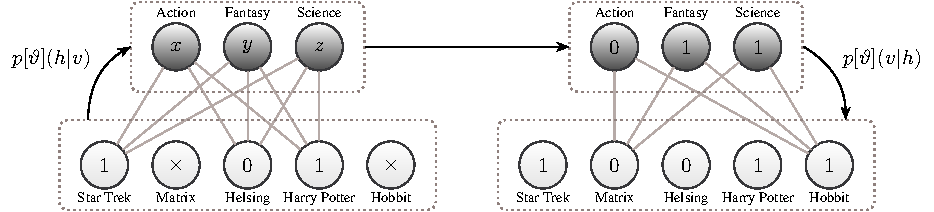
\includegraphics[width=0.9\textwidth]{figures/rbm-inference-example.pdf}
      \caption{%
        The figure shows a schematic example of the application of the inference process to the prediction of movie ratings for a given imaginary user.
        At first, only the rated movies will be used to sample hidden values.
        Then with respect to the sampled hidden values movie ratings for the unrated movies will be sampled and be understood as predictions.
      }
      \label{fig:rbm-inference-example}
    \end{figure*}

    The general inference for an RBM, that means sampling from the probability distribution, can be done by using Gibbs sampling explained in the section above.
    Here we will explicitly talk about the inference for the collaborative filtering problem of movie ratings from users.
    After talking about the model and the learning process of an RBM the inference process seems to be rather simple in some sense.
    Figure \ref{fig:rbm-inference-example} shows an example for this procedure.

    First, we get the vector of rated and unrated movies from a given user.
    We then have to sample the hidden values via the posterior probability by using only the values for the rated movies.
    After this we are now able to sample values for the unrated movies again by using the posterior probability with the previously sampled hidden values.
    These new sampled visible values are then taken to be the predictions of the user ratings.
  % section Inference (end)
\end{document}